\section{El problema del viajante de comercio}

\begin{frame}{Problema}
Hallar el recorrido con distancia mínima en un conjunto de
ciudades que pase por todas las ciudades y regrese al punto inicial.

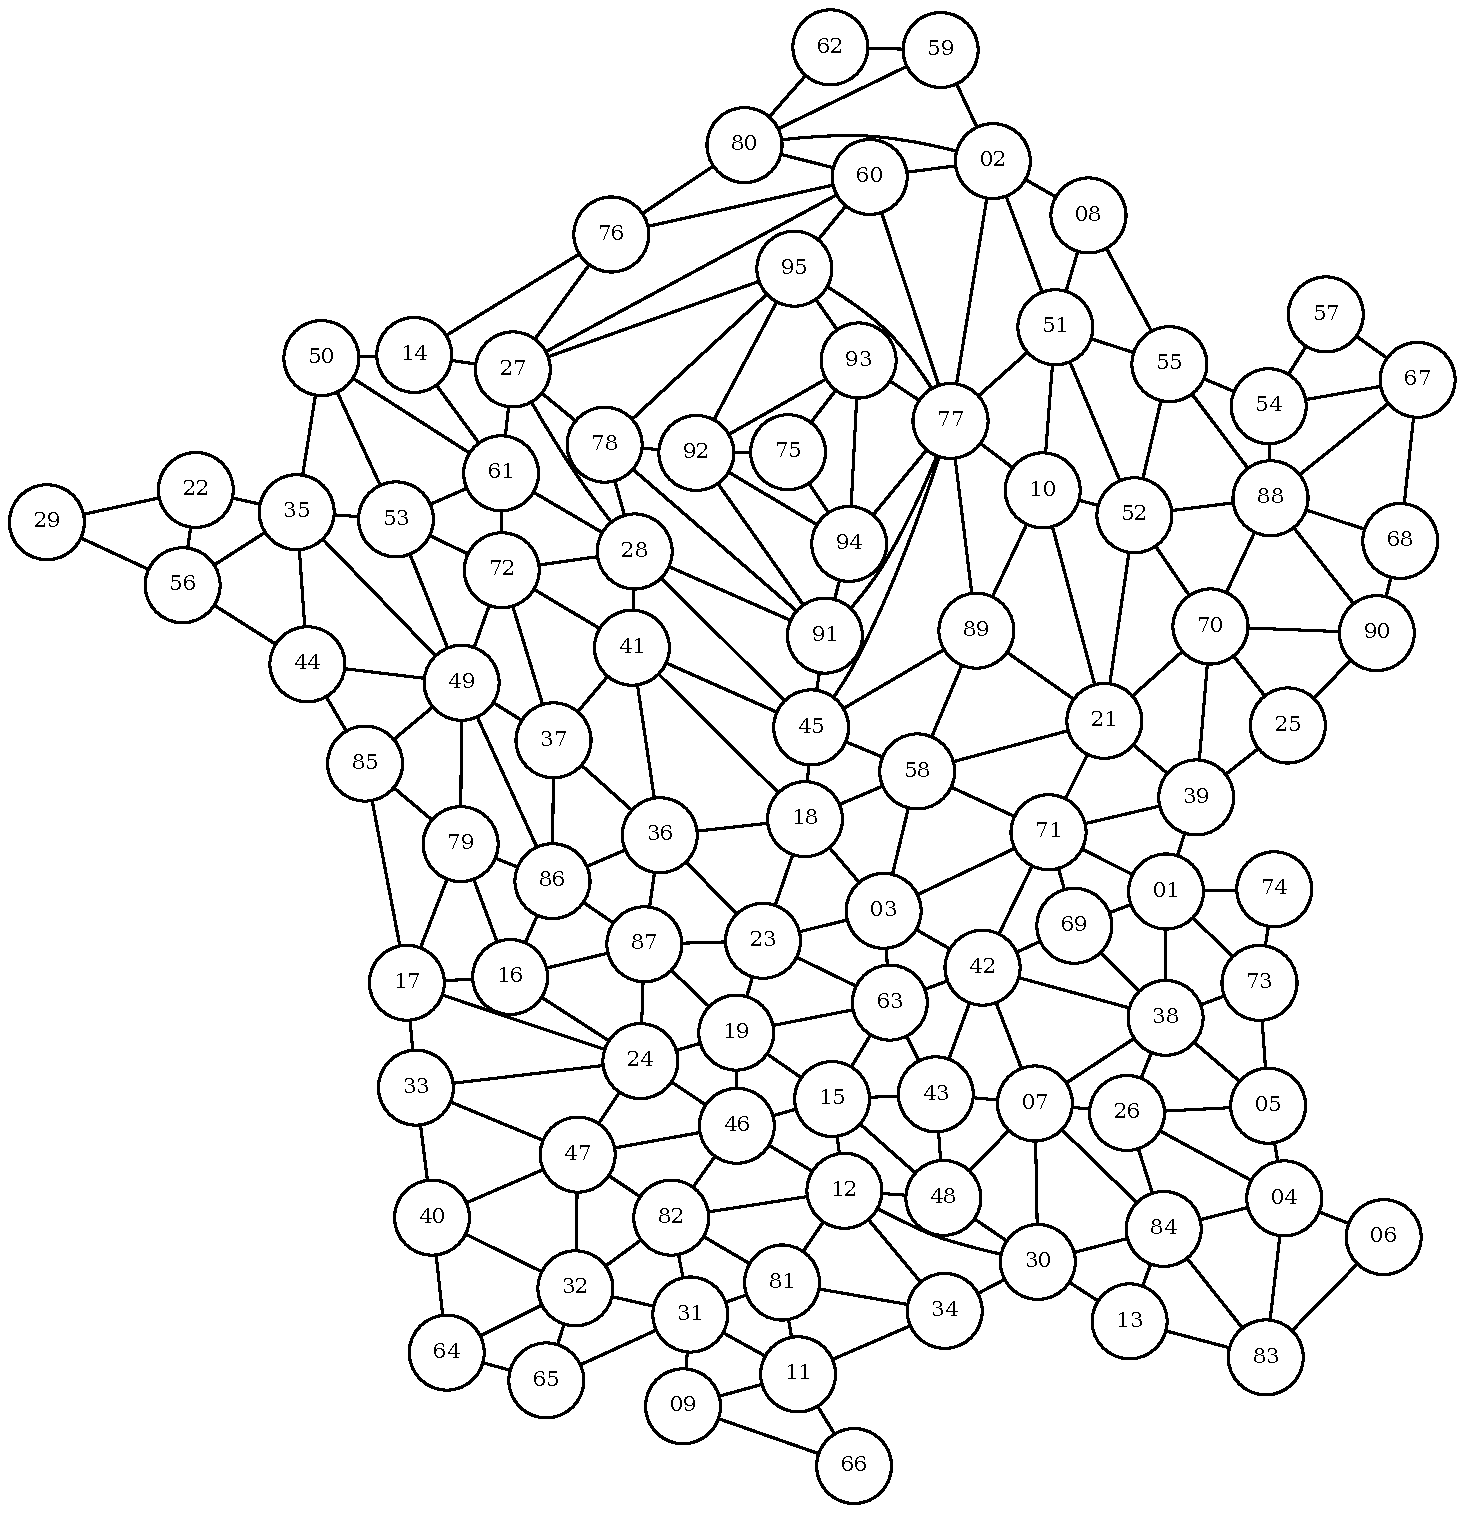
\includegraphics[width=.5\textwidth]{img/Francia} \centering
\end{frame}

\begin{frame}{Algoritmos}
\begin{description}
 \item[Entrada:] Ficheros con ciudades indicadas como puntos en el plano según sus
 coordenadas.
 \item[Salida:] \texttt{vector<int>} con el orden en el que se recorren las ciudades.
\end{description}
\end{frame}

\begin{frame}{Grafos}

Un grafo consta de:

\begin{itemize}
  \item Una \textbf{cantidad de nodos}, almacenada en el atributo \texttt{nodos}.
  \item Una \textbf{matriz de pesos}, almacenada en el vector \texttt{lados}.
\end{itemize}
\lstinputlisting[firstline=16, lastline=20]{cpps/grafo.h}
\end{frame}

\begin{frame}[fragile]{Construcción del grafo}
Construimos el grafo a partir de la distancia euclídea redondeada al entero más próximo.
Esto nos permite resolver problemas más generales.
\lstinputlisting[firstline=47, lastline=51]{cpps/grafo.h}
\end{frame}

\subsection{Algoritmos}

\begin{frame}[fragile]{Vecino más cercano}
Tomamos la ciudad inicial y almacenamos en las ciudades no visitadas:
\lstinputlisting[firstline=18, lastline=21]{cpps/tsp.cpp}
Devolveremos \texttt{trayecto}.
\end{frame}

\begin{frame}[fragile]{Vecino más cercano}
\vspace*{-.5cm}
Recorremos la lista buscando aquella ciudad con distancia mínima:
\lstinputlisting[firstline=23, lastline=37]{cpps/tsp.cpp}
\end{frame}

\begin{frame}{Inserción (algoritmo)}
  \begin{itemize}
    \item Toma las ciudades más al norte, este y oeste
    \item Para cada nodo, halla el índice que aumente menos el recorrido
    \item Inserta en dicho índice el nodo que aumente menos el recorrido
  \end{itemize}
\end{frame}

\begin{frame}[fragile]{Inserción (código)}
\vspace*{-.5cm}
\lstinputlisting[firstline = 95, lastline = 109]{cpps/tsp.cpp}
\end{frame}

\begin{frame}{Colonia de hormigas}
Este algoritmo se inspira en la comunicación por feromonas
de una colonia de hormigas para encontrar el camino mínimo hacia una fuente de comida.
%% TODO: Gráfico explicativo de las hormigas
\end{frame}

\begin{frame}{Colonia}
Una Colonia consta de:
\begin{itemize}
  \item Grafo de \textbf{distancias} entre las ciudades.
  \item Grafo con las \textbf{feromonas} de cada camino, inicialmente arbitrarias.
  \item Constantes $\alpha, \beta, \rho, C, P$.
\end{itemize}
\note{Explicar qué son las feromonas}
\end{frame}

\begin{frame}{Constantes}
\begin{description}
  \item[$\alpha$] Peso que tienen las feromonas.
  \item[$\beta$] Peso que tienen la distancias.
  \item[$\rho$] Coeficiente de evaporación de las feromonas.
  \item[$C$] Cuántas feromonas se añaden a un camino.
  \item[$P$] Probabilidad de tomar el camino más corto.
\end{description}
\note{Explicar cada constante}
\end{frame}

\begin{frame}{Comparativa de los algoritmos}
  %%TODO: Cosas
\end{frame}
